\documentclass[12pt]{report}
\usepackage[french]{babel}

\usepackage[T1]{fontenc}
\usepackage{amstext}
\usepackage{amssymb}
\usepackage{graphicx}
\usepackage[utf8]{inputenc}
\usepackage{babel}
\usepackage{hyperref}
\usepackage{float}
\usepackage{subcaption}



\usepackage[a4paper,top=3cm,bottom=2cm,left=2cm,right=2cm,marginparwidth=1.75cm]{geometry}  % pour configurer les marges


\makeatletter

\providecommand{\tabularnewline}{\\}

\makeatother

\begin{document}


\begin{titlepage}

\newcommand{\HRule}{\rule{\linewidth}{0.5mm}} % Defines a new command for the horizontal lines, change thickness here

\center % Center everything on the page
 
%----------------------------------------------------------------------------------------
%   HEADING SECTIONS
%----------------------------------------------------------------------------------------

\vspace{3cm}
\textsc{\LARGE Kévin REN,  Théo MASSA \\[0.5cm] Guillaume GARDE, Hugo HOFMANN } \\ [1.5cm]
\textsc{\Large UV 6.1 -- Projet au lac de Guerlédan}\\[1.5cm]

%----------------------------------------------------------------------------------------
%   TITLE SECTION
%----------------------------------------------------------------------------------------
\HRule \\[0.4cm]
{ \huge \bfseries \textsc{Docking\\[0.3cm]}}
\HRule \\[.5cm]

%----------------------------------------------------------------------------------------
%   DATE SECTION
%----------------------------------------------------------------------------------------

\vspace{1cm}
{\huge \today}\\[1cm] % Date, change the \today to a set date if you want to be precise

%----------------------------------------------------------------------------------------
%   LOGO SECTION
%----------------------------------------------------------------------------------------
% \raggedright
\vspace{2cm}
% 
\includegraphics[width = 5.5cm]{logo.pdf}\\[1cm] % Include a department/university logo - this will require the graphicx package

\includegraphics[width=6cm]{imgs/logo_ensta.jpg}

\includegraphics[width=6cm]{imgs/logo-lab-sticc2.png}

\includegraphics[width=6cm]{imgs/logo_ubs_transparent.png} 
%----------------------------------------------------------------------------------------

\vfill % Fill the rest of the page with whitespace

\end{titlepage}

\tableofcontents

\chapter{Introduction}

\section{Présentation du sujet}

Que ce soit dans le monde de la recherche ou dans les différents domaines dans lesquels sont utilisés les drones et tout particulièrement les AUV ou UAV, l'une des grandes difficultés rencontrées est très certainement celle du docking. En effet, bien qu'il faille tôt ou tard récupérer le drone à la fin de sa mission ou en cas de problème, cela peut se révéler dans le meilleur des cas fastidieux (dans le cas ou la manoeuvre est manuelle par exemple) et dans le pire des cas difficile voire dangereux pour le drone (dans le cas d'une mer agitée par exemple). Dans le cas d'une mission autonome loin du bateau, on comprend qu'il peut être très intéressant de développer une solution de docking autonome, permettant au drone de revenir vers sa base tout seul et avec précision. L'objectif de ce projet Guerlédan sera donc de développer cette solution en s'intéressant au cas d'un AUV sur le lac. Les objectifs seront les suivants:

\begin{enumerate}
    \item Le drone doit être capable de planifier et réaliser son retour vers le dock
    \item Le dock doit pouvoir communiquer sa position et son attitude en temps réel et potentiellement à longue distance pour que le drone puisse effectuer son retour peu importe la position (parfois changeante) du dock
    \item Le docking doit se faire avec une précision suffisante (à la dizaine de centimètres voire mieux) pour que le drone puisse correctement entrer dans la structure
\end{enumerate}

\section{Matériel à disposition}
La majorité du matériel nécessaire nous a directement été fournie. En voici une liste (non exhaustive).
\subsection{Dock}
Pour ce qui est du dock, nous avions déjà les éléments nécessaires :

\begin{itemize}
    \item Un récepteur GNSS \textit{Ublox} monté sur une carte \textit{ArduSimple}
    \item Une antenne radio \textit{Xbee} pour recevoir les corrections RTK
    \item Une IMU \textit{SBG Ellipse A}
    \item \textit{NVIDIA Jetson Nano avec ROS}
\end{itemize}

Quant à la structure en elle-même du dock, nos encadrants ont fourni pour la deuxième semaine d'expérimentations un dock \ref{fig:dock} permettant d'accueillir le drone.
Puisque la mission nécessite que le dock communique avec le drone, et ce à longue distance, nous avons également reçu deux modems \textit{Simpulse SL200}\ref{fig:simpulse} qu'il a fallu configurer.

\begin{figure}[H]
    \begin{subfigure}{0.45\textwidth}
        \centering
        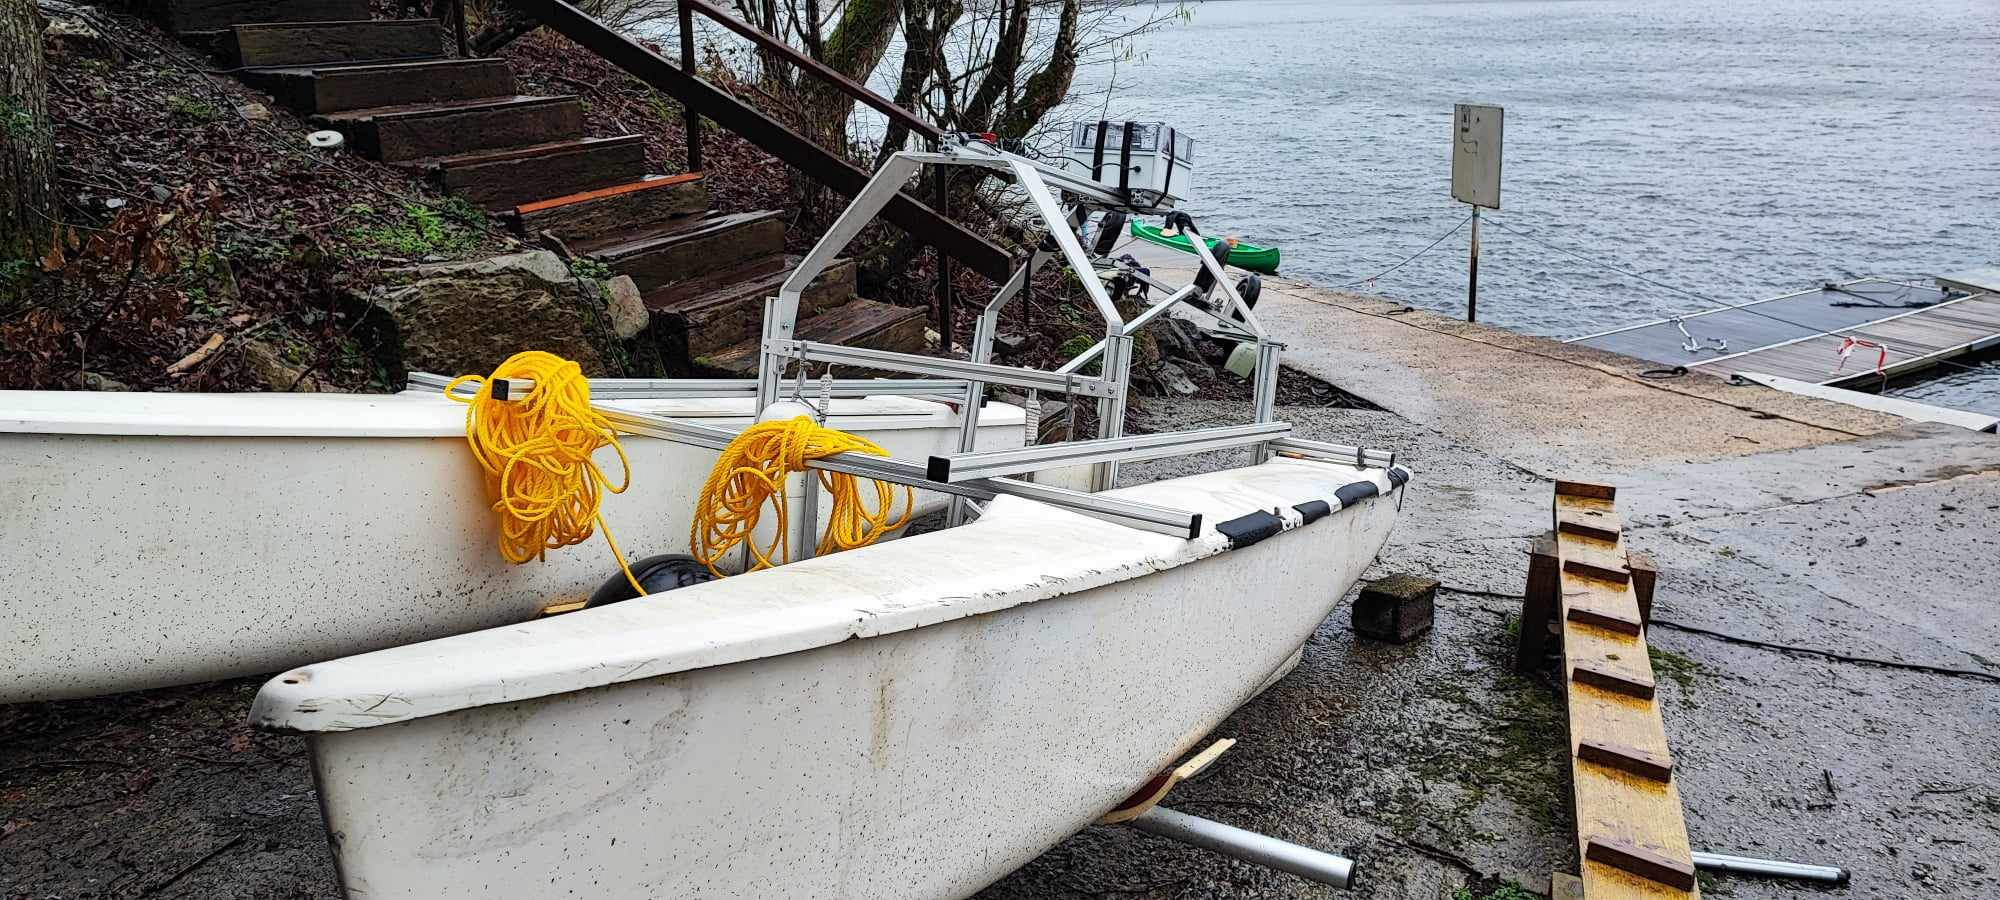
\includegraphics[width=0.8\textwidth]{imgs/dock.jpg}
        \caption{Le dock}
        \label{fig:dock}
    \end{subfigure}
    \begin{subfigure}{0.4\textwidth}
        \centering
        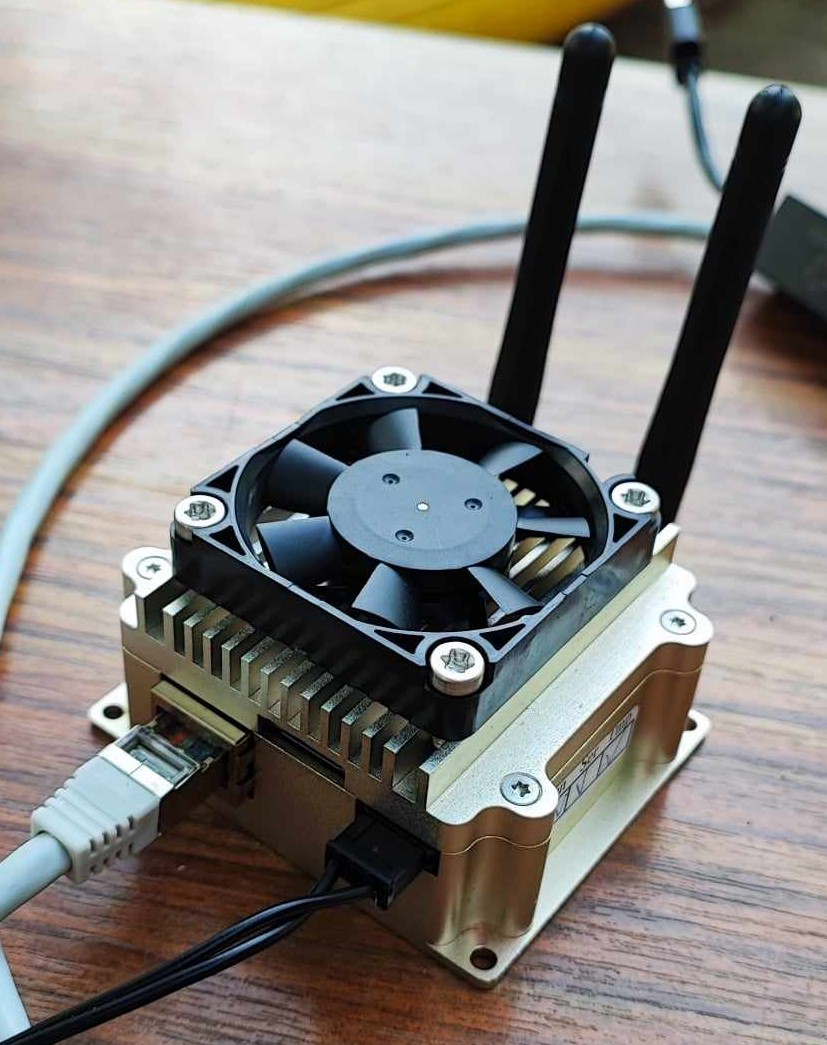
\includegraphics[width=0.4\textwidth]{imgs/simpulse.jpg}
        \caption{Modem Simpulse}
        \label{fig:simpulse}
    \end{subfigure}
    \caption{Matériel fourni}
\end{figure}

\subsection{Drone AUV}
Pour ce qui est de l'AUV, nous avons pu travailler (seulement le temps des deux semaines sur le lac) avec le \textit{M1800} d'\textit{IMSolutions}.
\begin{figure}[H]
    \centering
    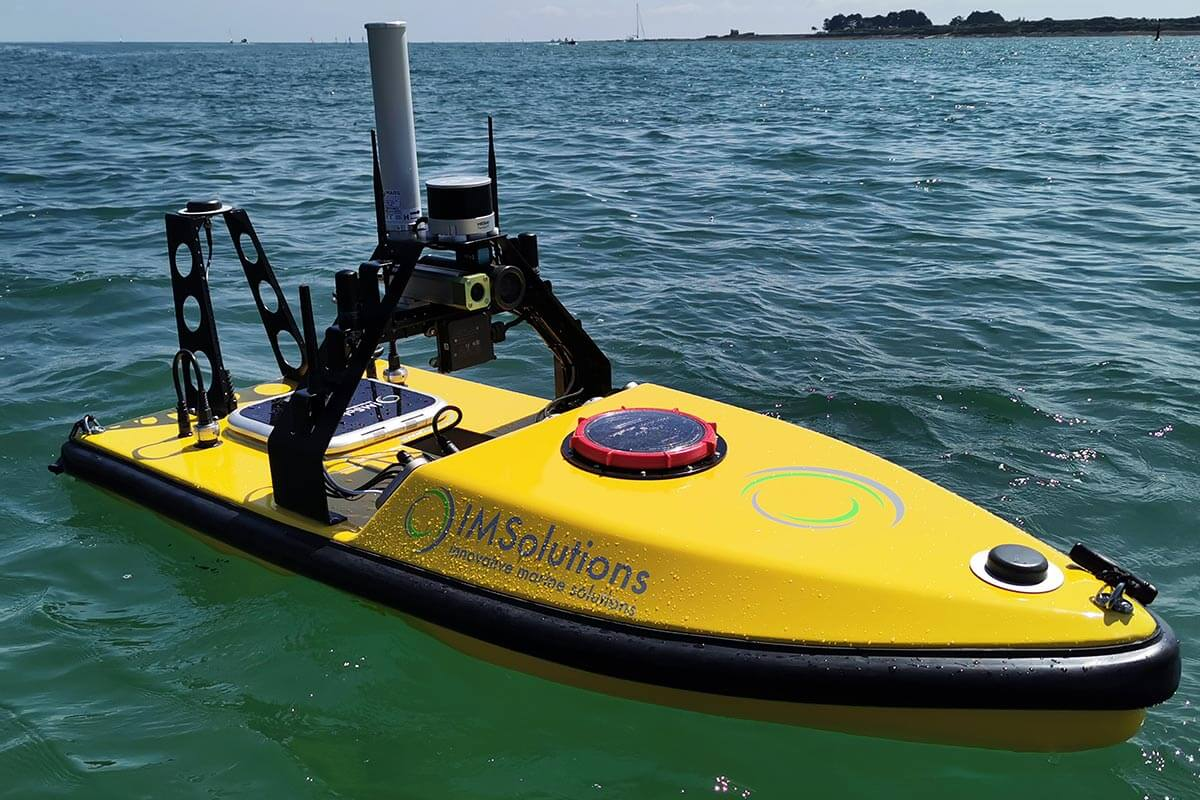
\includegraphics[width=0.5\textwidth]{imgs/monodrone-1800-chenal.jpg}
    \caption{L'AUV en question, sans les capteurs supplémentaires}
\end{figure}
Le drone embarque déjà tous les capteurs nécessaires à la mission comme elle a été envisagée :

\begin{itemize}
    \item Récepteur GNSS RTK
    \item IMU \textit{SBG Ellipse D}
\end{itemize}

Sur le modèle exact qui nous a été fourni, de nombreux autres capteurs tels que des caméras et un LIDAR ont été montés; s'ils n'ont pas été utilisés pendant la mission (dont le plus important était surtout dans un premier temps l'approche du drone vers le dock), ils pourraient en revanche se révéler utiles dans un second temps pour de prochaines expérimentations sur le projet.
\subsection{Rover}

Puisque le drone n'était disponible que peu de temps et uniquement lors des semaines à Guerlédan, nous avions besoin d'un remplacement pour pouvoir continuer à travailler et tester nos algorithmes à l'ENSTA. C'est pour cela que nous avons pu travailler avec l'\textit{AION R1}\ref{fig:rover}, un rover à la structure software équivalente à celle du drone (tournant sous \textit{ROS}, et gérant les commandes moteurs via une carte \textit{Pixhawk}). On peut ainsi commander le rover exactement de la même manière que l'AUV, c'est-à-dire dans notre cas lui envoyer des commandes en vitesses linéaire et angulaire.

\begin{figure}[H]
    \centering
    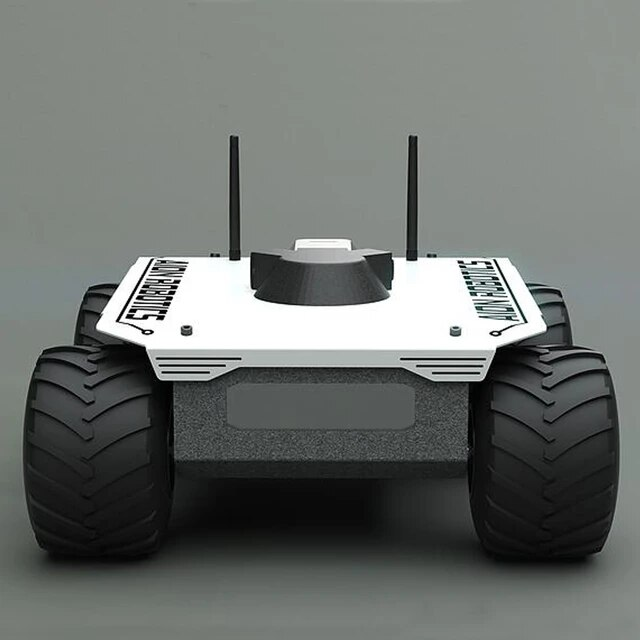
\includegraphics[width=0.4\textwidth]{imgs/rover.jpg}
    \caption{l'\textit{AION Robotics R1}}
    \label{fig:rover}
\end{figure}

\chapter{Conception du dock}
\section{Mise en place d'une base RTK}
Le positionnement GPS acquis par les capteurs à disposition confère une précision métrique, les signaux GPS étant perturbés par l'atmosphère. Or, il faut de meilleures performances pour espérer docker le drône dans un environnement confiné et restreint. 
L'idée était donc de mettre en place un système de positionnement plus précis (centimétrique dans l'idéal) en  utilisant le dispositif du \textit{Real Time Kinematic} (RTK).
Pour cela, il faut installer une base GPS fixe de position connue précisément. Elle servira de garde-fou en diffusant des corrections de positionnement aux systèmes GPS connectés.
L'installation est donc en deux parties, la première, à terre, l'autre, directement sur le dock.
\subsection{Capteurs à disposition}
L'acquisition de signaux GPS se fait grâce à deux modules \textit{ArduSimple} équipés de processeurs \textit{u-blox ZED-F9P}. 
% //TODO : images ?
Les deux modules communiquent grâce à leur antenne radio \textit{Xbee S2C 2,4 GHz}. La base dispose d'une antenne GPS qui permet une meilleure acquisition des signaux. 
Il est possible d'utiliser une \textit{Raspberry} pour configurer la base GPS en lui conférant une interface graphique. Un guide de configuration des capteurs est disponible en annexe.
% //TODO : guide rtk en annexe
\subsection{Installation de la base}
L'installation de la base peut se faire de deux manières différentes. 
\begin{enumerate}
    \item 
\end{enumerate}
\subsection{Configuration du dock}

\section{Mise en place du dock}

\section{Communication avec le reste du système}

\chapter{Stratégie d'approche de docking}

\section{Modèle cinématique}

\section{Filtre de Kalman}

\section{Algorithme de Kévin}

\chapter{Architecture logicielle}

\chapter{Essais à Guerlédan}

\section{Première semaine}

La première semaine d'expérimentations au lac de Guerlédan, du 9 au 13 octobre 2023, fut davantage une semaine de découverte du projet et permit une première approche à la résolution de notre problème. 
Durant cette semaine, nous avons rencontré nos encadrants et pris en main le matériel que nous avions à notre disposition, c'est à dire principalement les composants de ce qui sera plus tard notre dock,
que nous avons conçu durant cette semaine. Ainsi, à l'aide des composants décrits précédemment, nous avons été capable de créer la boite qui contient les capteurs nécessaires au bon fonctionnement du dock. 

D'autre part, nous travaillions en parallèle sur la mise en place de la correction RTK en configurant les différentes cartes et en prenant des mesures nécessaires au calcul de la correction. 

Enfin, une première version simplifiée de l'architecture logicielle a commencée à être implémentée. 

La principale problématique de cette semaine, qui est la même que celle rencontrée durant la période séparant cette semaine de la seconde, est l'impossibilité d'expérimenter directement sur l'AUV qui 
est le drone principal de notre sujet. En effet, l'avancée de notre projet ne nous permettait pas la sécurité de pouvoir tester nos algorithmes de manière sereine sur le drone et nous avons également 
rencontré quelques difficultés avec l'utilisation de l'interface MAVROS, qui fait le lien entre notre architecture ROS et MAVLink. Le principal problème résidait dans le fait qu'il semblait que MAVLink 
avait en mémoire des waypoints GPS que le drone tentait de rejoindre en priorité avant de prendre en compte nos commandes. Cela empêchait toute exploitation du drone en mode automatique, ce qui est nécessaire
au bon fonctionnement de nos algorithmes.

Heureusement ce problème avait tout le temps d'être réglé, étant donné que nous n'utiliserions pas le drone d'içi à la seconde semaine d'expérimentation à Guerlédan, en février 2024. De plus, nous avons 
décidé de concentrer nos efforts à la mise en place et la conversion de nos algorithmes pour la mise en place sur le Rover qui nous sert de remplacement au drone et qui nous sert de moyen d'expérimentations à l'école. 


\section{Deuxième semaine}

La seconde semaine d'expérimentations, qui eut lieu du 5 au 9 février 2024, fut bien davantage une semaine d'expérimentation que la première. 
En effet, forts du travail effectué entre les deux semaines, nous avons été capables de mettre en oeuvre et tester nos algorithmes sur le drone principal.

La première étape préliminaire à cela fut de convertir nos codes, conçus pour fonctionner sur le rover, pour qu'ils puissent se mettre correctement en oeuvre sur le drone, qui, on le rappelle, n'est pas
équipé des mêmes capteurs et architecture logicielle des drivers. Il y a également des fonctionnalités supplémentaires sur le drone qui permettent plus de précision sur l'acquisition de l'état du drone, notamment 
l'obtention du \textit{True Heading}, sur lequel nous reviendrons plus tard, qui permet l'obtention du cap avec une plus grande fiabilité qu'en utilisant uniquement la centrale inertielle. 

Une des principales problématiques rencontrées durant la semaine réside dans la difficulté à bien calibrer les centrales inertielles. En effet, les centrales inertielles SBG nécessitent une étape de calibration
afin qu'elles compensent le champ magnétique disturbé pour calculer son attitude. Malgré de nombreux essais dans de nombreuses configurations, nous n'avons jamais réussi à bien configurer la centrale 
pour que la sortie de son filtre de Kalman concernant le cap ne diverge pas, surtout pour le dock. Si le dock reste trop longtemps immobile, sans perturbations, son cap se met à diverger rapidement.
Ce problème reste un point d'amélioration essentiel car il est une des raisons principales à l'absence d'expérimentations avec le vrai dock. 

Cependant, nous avons développé des alternatives permettant tout de même de mettre en oeuvre nos algorithmes en contournant le problème. Lorsque nous lancons le système, nous avons le choix entre
utiliser le vrai dock ou un dock simulé. Le dock simulé repose soit sur des logs d'essais précédents soit sur une position et orientation désirée précisées au lancement. 
En faisant cela, nous avons été capable de tester et prouver la robustesse de nos algorithmes, même sans présence d'un vrai

\chapter{Conclusion}
\section{Résultats}

\section{Perspectives}
%//TODO mentionner : + de tests avec le vrai dock, approche avec d'autres capteurs (LIDAR, caméra)
   



\bibliographystyle{plain}
\bibliography{mabiblio}

\end{document}
